\documentclass{article}
\usepackage[T1]{fontenc}
\usepackage{lmodern}
\usepackage{graphicx}
\usepackage{amsmath,amssymb}
\usepackage[a4paper,margin=2cm]{geometry}
\usepackage[absolute,overlay]{textpos}
\setlength{\TPHorizModule}{1mm}
\setlength{\TPVertModule}{1mm}
\usepackage[indonesian]{babel}
\usepackage{hyperref}
\setlength{\emergencystretch}{2em}
% unit: Halaman 85

\begin{document}

% === Halaman 85 (llm) ===

\begin{itemize}
  \item Contoh:
  \begin{itemize}
    \item misalkan bigram yang sering muncul di dalam cipherteks adalah BM.
    \item bigram yang sering muncul di dalam bahasa Inggris adalah TH
    \item jadi, kita duga TH dipetakan menjadi BM
    \item misalkan TH dienkripsi dengan aturan segiempat, maka jika T dan H membentuk segiempat dengan B dan M, maka posisi mereka harus konsisten dalam matriks.
    \item Artinya: T satu baris dengan B, dan H satu baris dengan M
  \end{itemize}
\end{itemize}

\vspace{15mm}

\begin{itemize}
  \item Jika TH dienkripsi dengan aturan kolom, maka B di bawah T, M di bawah H
  \item Jika TH dienkripsi dengan aturan baris, maka B di kanan T, M di kanan H
  \item Mulai bangun matriks parsial $5 \times 5$ dengan hipotesis seperti di atas
\end{itemize}

% deskripsi: Ilustrasi posisi huruf T, B, M, dan H yang membentuk segiempat dalam matriks
% bbox normalisasi: [0.2100, 0.5500, 0.3200, 0.7400]
\begin{textblock*}{23.10mm}(44.10mm,163.35mm)
\noindent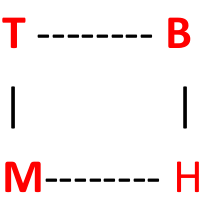
\includegraphics[width=23.10mm,height=56.43mm]{../../images/llm/page_085_img_01.png}%
\end{textblock*}

\end{document}
